% ME3050 -  Dynamics Modeling and Controls - Tennessee Technological University
% Tristan Hill - Spring 2020 - Summer 2020 - Spring 2022
% Dynamics Modeling and Controls
% Lecture Module - Laplace Transforms - Topic 2  - Laplace Transforms Method 

% Document settings

%\documentclass{beamer}                  % for presentation ?
\documentclass[handout]{beamer}  % for handout ?

\usepackage{../dmc_lectures} % .sty in parent folder

%\newcommand{\MNUM}{10\hspace{2mm}} % Module number
\newcommand{\TNUM}{2\hspace{2mm}} % Topic number 
\newcommand{\moduletitle}{The Laplace Transform} % Titles and Stuff
\newcommand{\topictitle}{Laplace Transforms Method} 

\newcommand{\sectiontitleI}{Step 1 - Apply Laplace Transform} % More Titles and Stuff
\newcommand{\sectiontitleII}{Step 2 - Solve for $X(s)$}
\newcommand{\sectiontitleIII}{Step 3 - Rearrange to Find Invertable Form}
\newcommand{\sectiontitleIV}{Step 4 - Invert for Final Answer}

\author{ME3050 - Dynamic Modeling and Controls}
\title{Lecture Module - \moduletitle}
\date{Mechanical Engineering\vspc Tennessee Technological University}

\begin{document}
	
	\lstset{language=MATLAB,basicstyle=\ttfamily\small,showstringspaces=false}
	
	\frame{\titlepage \center\begin{framed}\Large \textbf{Topic \TNUM - \topictitle}\end{framed} \vspace{5mm}}
	
	% Section 0 - Outline
	\frame{
		
		\large \textbf{Topic \TNUM - \topictitle} \vspace{3mm}\\
		
		\begin{itemize}
			
			\item \sectiontitleI    \vspc % Section I
			\item \sectiontitleII 	\vspc % Section II
			\item \sectiontitleIII 	\vspc %Section III
			\item \sectiontitleIV 	\vspc %Section IV
			%\item \sectiontitleV 	\vspc %Section V
			
		\end{itemize}
		
	}
	


\section{\sectiontitleI}

\frame{
\frametitle{\sectiontitleI}

Example:

Solve the first order differential equation using the Laplace Transforms Method with the initial condition given. 
\[4\dot{x}=sin\left(t\right) \hspccc with \hspccc x\left(t=0\right)=x_0 \] 
Apply the Laplace Transform to both sides of the differential equation. 

\[ 4\left(sX\left(s \right)-x_0 \right)=\frac{1}{s^2+1} \]

}

\section{\sectiontitleII}
\frame{
\frametitle{\sectiontitleII}
This step can seem open ended...
\[X(s)=\frac{1}{4s\left(s^2+1\right)}+\frac{x_0}{s} \] 

}

\section{\sectiontitleIII}
\frame{
\frametitle{\sectiontitleIII}

Write $X\left(s\right)$ in a form that can be inverted using the table of Laplace transform pairs. This typically involves partial fraction decomposition. 
\[\frac{1}{4s\left(s^2+1 \right)}=\frac{1/4}{s\left(s^2+1\right)} =\frac{a}{s}+\frac{bs+c}{s^2+1} \] 

Mulitply through by the denominator $4s\left(s^2+1\right)$:
\[ 1=4as\left(s^2+1\right)+4s\left(bs+c\right)=4\left(a+b \right)s^2 + 4cs +4a \]

Solve for the coefficients by {\it equating coefficients}.

\[ \left( a+b\right)=0 \hspcc c=0 \hspcc a=\frac{1}{4} \implies a=\frac{1}{4} \hspcc b=-\frac{1}{4} \hspcc c=0 \]
}

\section{\sectiontitleIV}
\frame{
\frametitle{\sectiontitleIV}

Substitute the coefficients into $X(s)$,

\[ X(s) =\frac{x_0}{s}+\frac{1}{4s}-\frac{s}{4\left(s^2+1\right)} \]

and use the inverse transform to solve for $x(t)$. Use the Table.

\[ \Lagr^{-1} \left( X\left( s\right)\right)=x(t)= \]
\[ = x_0+\frac{1}{4}-\frac{1}{4}cos\left(t\right)=x_0+\frac{1}{4}\left(1-cos\left(t\right) \right) \]

This method works for complex problems but it can get messy...
}

\section{---}
\frame{
\frametitle{---}

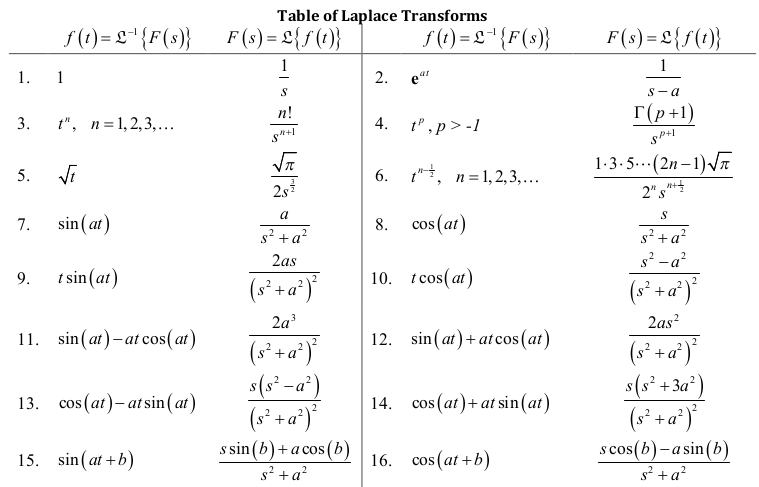
\includegraphics[scale=.35]{laplace_table_part1.png}


}

\frame{
\frametitle{---}

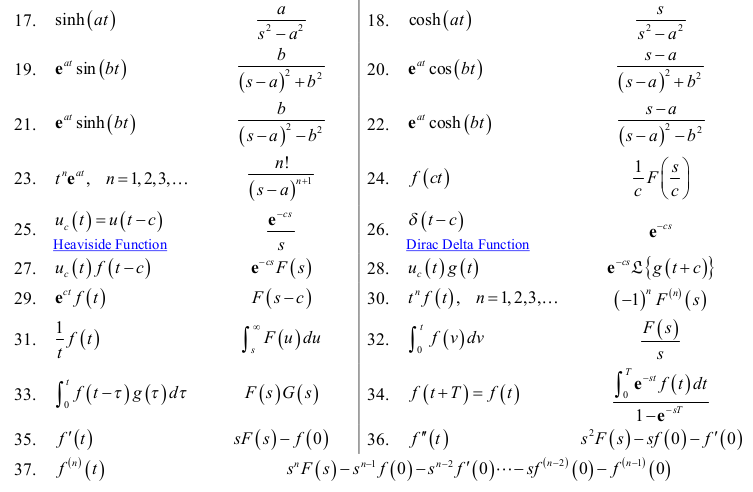
\includegraphics[scale=.35]{laplace_table_part2.png}


}

\end{document}

